\section{Цель работы}
	Реализовать многоагентную систему на выбранном фреймворке.
	
\section{Описание фреймворка}

	\textbf{JADE} – это программное обеспечение промежуточного слоя, разработанное компанией \href{http://jade.tilab.com}{TILAB} на языке Java, предназначенное для создания  распределенных мультиагентных приложений на основе транспортной архитектуры «точка-точка». И интеллект, и инициатива, и информация, и ресурсы, и контроль могут быть полностью распределены по мобильным терминалам также как и по компьютерам выделенной сети. Среда может динамично взаимодействовать  с узлами, которые в терминологии JADE называются агентами. Агенты то появляются, то исчезают  в системе в соответствии с потребностями и требованиями программной среды.   Коммуникации между узлами не зависят от типа сети (проводная, беспроводная). Они являются полностью симметричными, и каждый узел может, как инициировать запросы, так и отвечать на них.
	
	Платформа JADE включает как программные библиотеки (т.е. наборы Java-классов), требуемые для разработки прикладных агентов, так и среду исполнения, которая предоставляет базовые службы и которая должна быть активна на устройстве до того, как на нем будет исполняться агент. Каждый экземпляр JADE во время исполнения называется контейнером (так как он «содержит» агентов). Набор всех контейнеров называется платформой и предоставляет однородный слой, который прячет от агентов(а также от разработчиков приложений) сложность и распределенный характер механизмов, расположенных на более низком уровне(аппаратное обеспечение, операционные системы, типы сетей, JVM).
	
	\begin{figure}[ht] 
		\center
		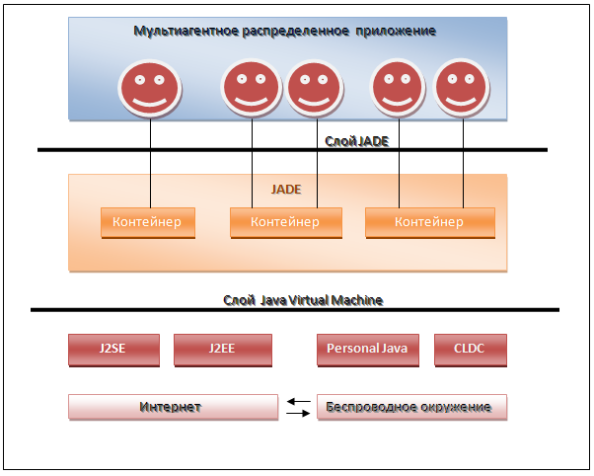
\includegraphics [width=0.6\textwidth] {jade}
		\caption{Архитектура JADE} 
	\end{figure}
	\FloatBarrier
	
	С  функциональной точки зрения программный инструмент JADE предоставляет базовые службы, необходимые для распределенных приложений типа «точка-точка» в стационарных и мобильных средах. Он позволяет каждому агенту динамически обнаруживать других агентов и обмениваться с ними сообщения в соответствии с парадигмой систем «точка-точка». С точки зрения приложения каждый агент идентифицируется уникальным именем и предоставляет набор служб. Он может регистрировать и модифицировать свои службы и/или искать агентов, предоставляющих данные службы. Также агент способен контролировать свой жизненный цикл и, в частности, общаться с другими агентами.
	
	Агенты общаются путем обмена асинхронными сообщениями, модель коммуникаций почти повсеместно применима для распределенных и слабосвязанных коммуникаций, т.е. коммуникаций между гетерогенными сущностями, который ничего не знают друг о друге. Для осуществления коммуникации агент только посылает сообщение получателю. Идентификатором служит имя агента(нет необходимости указывать ссылку на объект-получатель) и, как следствие, нет временной зависимости между общающимися агентами. Не требуется, чтобы отправитель и получатель были запущены в одно и тоже время. Получатель даже может не существовать(или еще не существовать) или может быть не известен явно отправителю. Отправитель может определить свойство отправителя (например, «все заинтересованные в футболе агенты»), чтобы указать конечный адрес.
	
	Платформа также содержит службу имен (которая проверяет, что каждый агент имеет уникальное имя) и службу «желтых страниц», которая может быть распределена по нескольким хостам. Можно создать графы федерации, чтобы определить организованные области агентных служб.  Другая очень важная функция заключается в доступности богатого набора графических инструментов, поддерживающих и стадию отладки, и стадию управления/наблюдения жизненного цикла приложения.  Посредством этих инструментов стало возможно удаленно управлять агентами (даже в том случае, когда они уже развернуты и запущены): могут быть сымитированы переговоры агентов, можно просматривать сообщения, которыми обмениваются агенты, можно заниматься мониторингом задач, контролировать жизненный цикл агента.

\section{Листинг}

	В процессе реализации создана следующая архитектура системы:
	\begin{figure}[ht] 
		\center
		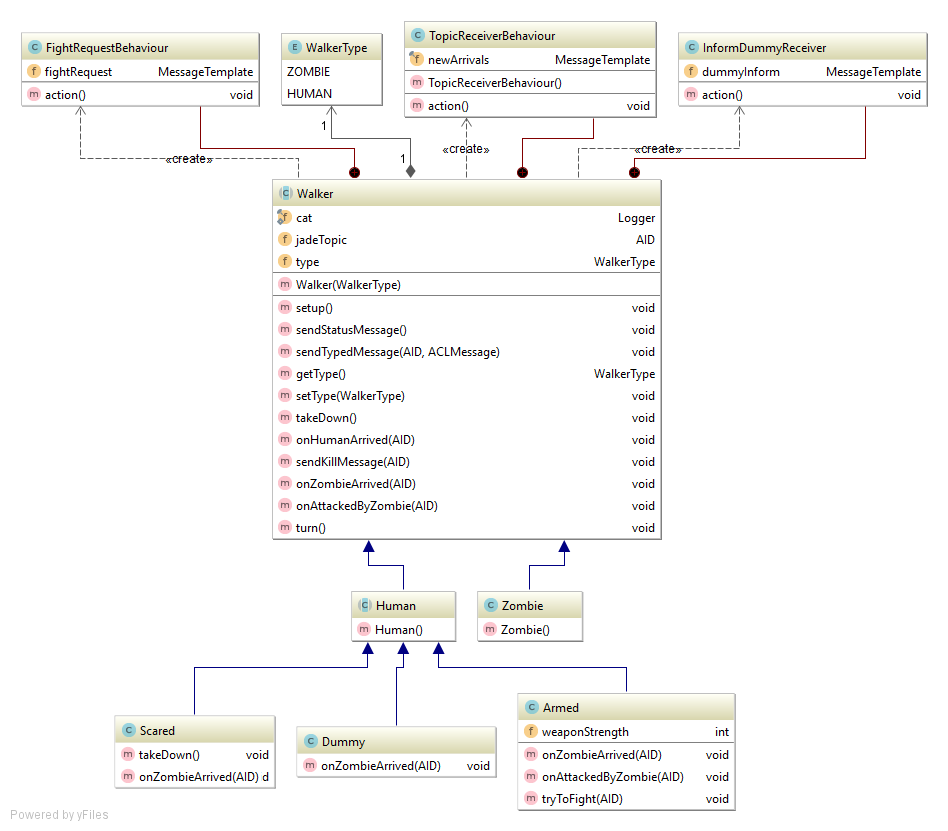
\includegraphics [width=0.6\textwidth] {diagram}
		\caption{Диаграмма классов} 
	\end{figure}
	\FloatBarrier
	
    \lstinputlisting[language={Java},caption={Базовый агент Walker и его поведения.}]{listings/Walker.java}
    
    \lstinputlisting[language={Java},caption={Типы Ходячих.}]{listings/WalkerType.java}
    
    \lstinputlisting[language={Java},caption={Зомби.}]{listings/Zombie.java}
    
    \lstinputlisting[language={Java},caption={Человек.}]{listings/Human.java}
    
    \lstinputlisting[language={Java},caption={Человек незнающий.}]{listings/Dummy.java}
    
    \lstinputlisting[language={Java},caption={Человек Знающий.}]{listings/Scared.java}
    
    \lstinputlisting[language={Java},caption={Защитник человечества.}]{listings/Armed.java}
	

\section{Пример работы системы}
